\section{解析してみよう}
\subsection{データの読み込み}
データを格納しているファイル:CSV(カンマ区切りテキスト)やTSV(タブ区切りテキスト)などを読み込む関数がある.
\begin{screen}
\begin{verbatim}
dataA=read.csv(file,header=TRUE,sep=",", skip=0, ...) 
dataB=read.table(file,header=FALSE,sep="",skip=0,...) 
\end{verbatim}
\end{screen}

使用するデータがCSVの場合は{\tt read.csv}関数を使用すればよい.スペース区切りなら{\tt read.table}関数,タブ区切りなら{\tt read.table(file,sep="\verb+\+t")}とする.

また,{\tt header}はテキストにタイトル行がある場合に指定し,{\tt skip}はデータの最初の行にコメント行がある場合読み飛ばす行数を指定する.

{\tt file}の部分はファイルのパスを指定する.面倒な場合は,{\tt file.choose()}とすることでファイルを選択できる.

ちなみに\verb+read.csv+は\verb+read.table+の引数が指定されたエイリアスです.
\begin{screen}
\begin{verbatim}
dataA=read.csv(file.choose()) # ファイル選択ウィンドウが表示される.
\end{verbatim}
\end{screen}
\subsection{データの書き出し}
データの読み込みがあるのでもちろんデータの書き出しもできます.
汎用性の高い形式からR独自の形式までいろいろあります.
解析の途中で一度Rを閉じる場合でもデータなどを残しておけばあっという間に復帰できます.
\subsubsection{CSV (主にテキスト)}
\begin{screen}
\begin{verbatim}
write.csv(オブジェクト名, file = "ファイル名.csv", quote = FALSE,
    sep = ", ", row.names = FALSE, colnames = TRUE)
\end{verbatim}
\end{screen}
こちらも\verb+write.table+のエイリアスで,基本的には互換性の高いCSVでの出力用のオプションとなっている.\verb+quote+は値を「"」で囲むかどうか,\verb+sep+は区切り文字,あとは列名行名を出力するかどうかのboolean.

\subsubsection{バイナリデータ(R専用)}
\begin{screen}
\begin{verbatim}
save(オブジェクト, file = "ファイル名.Rdata")
\end{verbatim}
\end{screen}
バイナリデータなのでテキストエディタでは編集できず,Rでしか読み込めない.生成されたファイルは\verb+load+関数かRにドラッグ・アンド・ドロップすれば元の変数名のまま読み込まれる.

\subsubsection{テキストデータ(R専用)}
\begin{screen}
\begin{verbatim}
dump(list, file="ファイル名.R", append=FALSE)
\end{verbatim}
\end{screen}
こちらもR専用のデータ形式.中身はテキストデータで表現され,編集可能.Rの命令として書き出される.\verb+source+関数かRにドラッグ・アンド・ドロップすれば元の変数名のまま読み込まれる.
便宜上\verb+list+としているが,\verb+"オブジェクト名"+とすれば良い.
\verb+append+は既にファイルが存在する場合に後ろに追記するか上書きするかのbooleanである.
\subsection{回帰分析}
統計的な解析をするうえで,線形回帰分析というものがある.これはデータ$X$とデータ$Y$がどのような関係にあるのかを定量的に式であてはめて分析する手法である.つまり,$Y$を目的変数,$X$を説明変数として,次の式を考える.
\begin{eqnarray*}
Y&=&\alpha +\beta X
\end{eqnarray*}

このように$Y$を$X$で説明するため,最小二乗法という,推定値と観測されたデータの差(残差)の2乗和が最も小さくなる推定を行う.本稿ではデータを生成して,回帰分析を行う.
\begin{breakbox}
\begin{verbatim}
> x2=rnorm(60)
> y2=runif(60,2,4)*x2
> plot(x2,y2)
\end{verbatim}
\begin{center}
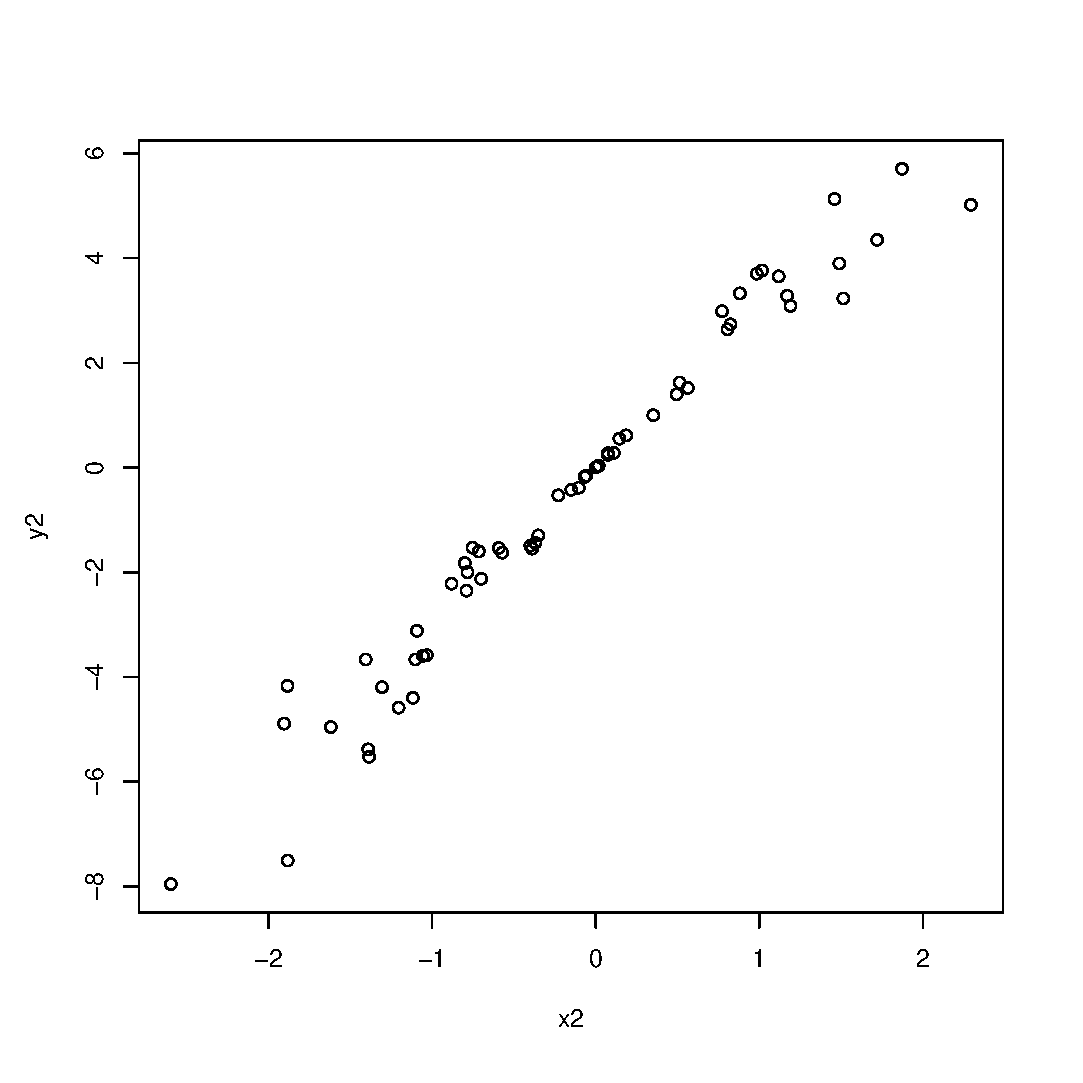
\includegraphics[width=8.2cm]{img/plot2.eps}
\end{center}
\begin{verbatim}
> result2=lm(y2~x2)
> result2

Call:
lm(formula = y2 ~ x2)

Coefficients:
(Intercept)           x2  
   -0.07254      2.98732  
\end{verbatim}
\end{breakbox}
この場合,回帰式は
\begin{eqnarray*}
Y&=&-0.07254-2.98732X
\end{eqnarray*}
となる.この回帰直線を赤線でプロットしたものが以下である.
\begin{breakbox}
\begin{verbatim}
> abline(result2,col=2,lwd=2)
\end{verbatim}
\begin{center}
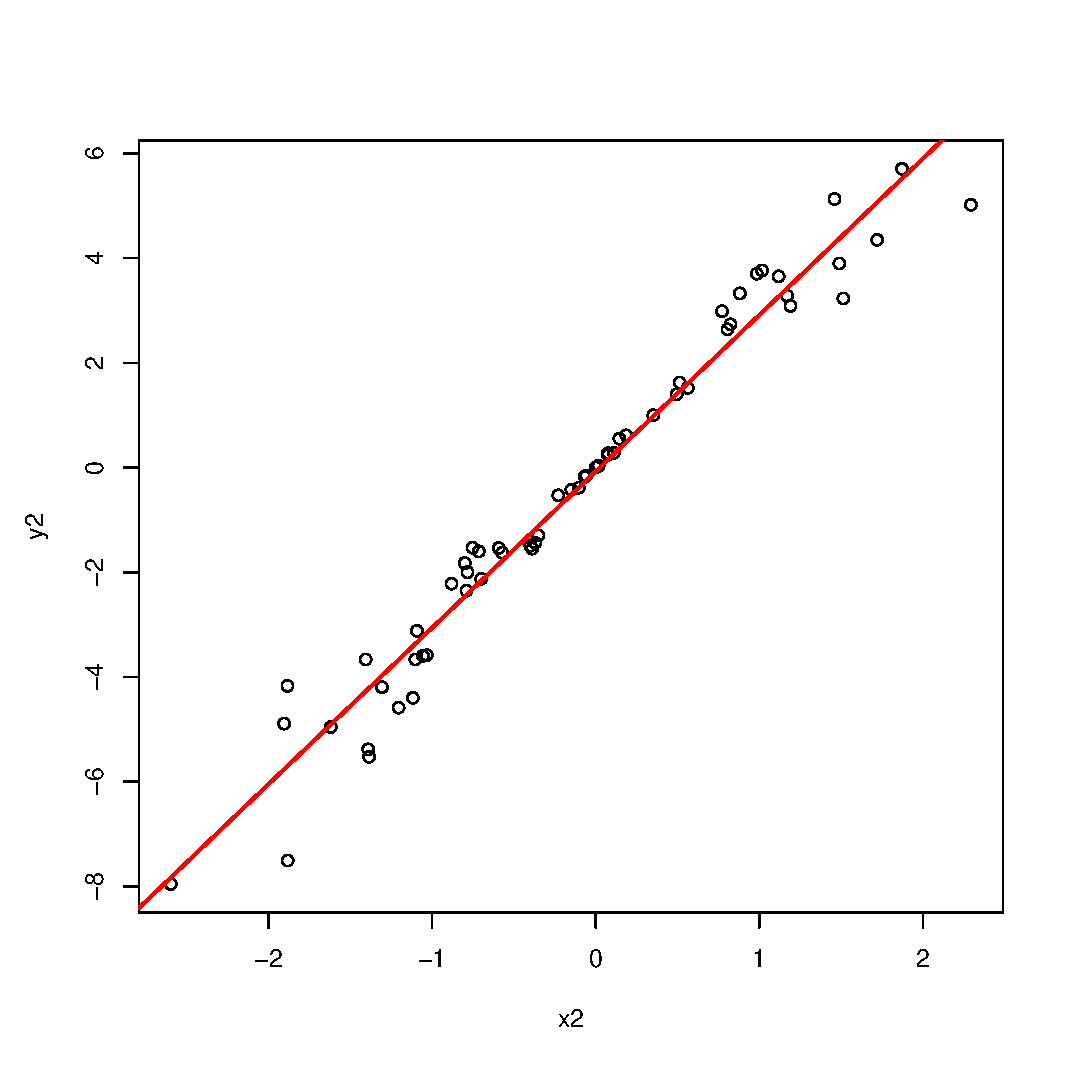
\includegraphics[width=8.2cm]{img/abline2.eps}
\end{center}
\end{breakbox}
また,回帰分析では,係数が$0$と有意に異なるかどうかの検定を行い,係数に意味があるのかを確認する.

{\large 帰無仮説$H_0$:$\beta=0$

対立仮説$H_1$:$\beta \ne 0$}

このような,仮説を立てて帰無仮説が棄却されるかを調べる.
\begin{breakbox}
\begin{verbatim}
> summary(result2)

Call:
lm(formula = y2 ~ x2)

Residuals:
     Min       1Q   Median       3Q      Max 
-1.80981 -0.23454  0.07632  0.31896  1.53236 

Coefficients:
            Estimate Std. Error t value Pr(>|t|)    
(Intercept) -0.07254    0.08324  -0.871    0.387    
x2           2.98732    0.07784  38.380   <2e-16 ***
---
Signif. codes:  0 ‘***’ 0.001 ‘**’ 0.01 ‘*’ 0.05 ‘.’ 0.1 ‘ ’ 1 

Residual standard error: 0.6383 on 58 degrees of freedom
Multiple R-squared: 0.9621,     Adjusted R-squared: 0.9615 
F-statistic:  1473 on 1 and 58 DF,  p-value: < 2.2e-16 
\end{verbatim}
\end{breakbox}
この分散分析表を改めて書きなおしたものが以下である.
\begin{description}
\item[入力された式] \mbox{}\\
\verb+y2 ~ x2+
\item[残差の分布]\mbox{}\\
\begin{tabular}{ccccc}
\noalign{\hrule height 1pt}
最小値&25\%点&中央値&75\%点&最大値\\ \hline
-1.80981&-0.23454&0.07632&0.31896&1.53236 \\
\noalign{\hrule height 1pt}
\end{tabular}
\item[係数]\mbox{}\\
\begin{tabular}{rrrrrl}
\noalign{\hrule height 1pt}
    &\multicolumn{1}{c}{推定値}&\multicolumn{1}{c}{標準誤差}&\multicolumn{1}{c}{t値}&\multicolumn{1}{c}{P-値($Pr( t_0>|t|)$)}& \\ \hline
切片&-0.07254& 0.08324&-0.871&0.387& \\
  x1&2.98732&  0.07784& 38.380 &$<2\times 10^{-16}$ &*** \\
\noalign{\hrule height 1pt}
\end{tabular}

*** は有意水準0.001で有意であるということ.\\
有意水準0.001で帰無仮説$H_0$:$\beta=0$が棄却された.P-値が$<2\times 10^{-16}$とは帰無仮説が正しいときに,帰無仮説を棄却する確率が$2\times 10^{-16}$以下ということである.
\item[回帰統計]\mbox{}\\
\begin{tabular}{lr}
\noalign{\hrule height 1pt}
標準誤差&0.6282(自由度58)\\
決定係数$R^2$&0.9621\\
自由度調整済決定係数$R^2$&0.9615\\
F値(観測された分散比)&1473(自由度1と58)\\
P-値&$<2\times 10^{-16}$\\
\noalign{\hrule height 1pt}
\end{tabular}

ここのP-値ではすべての係数が0であるという帰無仮説の検定となっている.
\end{description}

次に,バラバラなデータを解析する.
\begin{breakbox}
\begin{verbatim}
> x1=rnorm(60)
> y1=rnorm(60)
> plot(x1,y1)
\end{verbatim}
\begin{center}
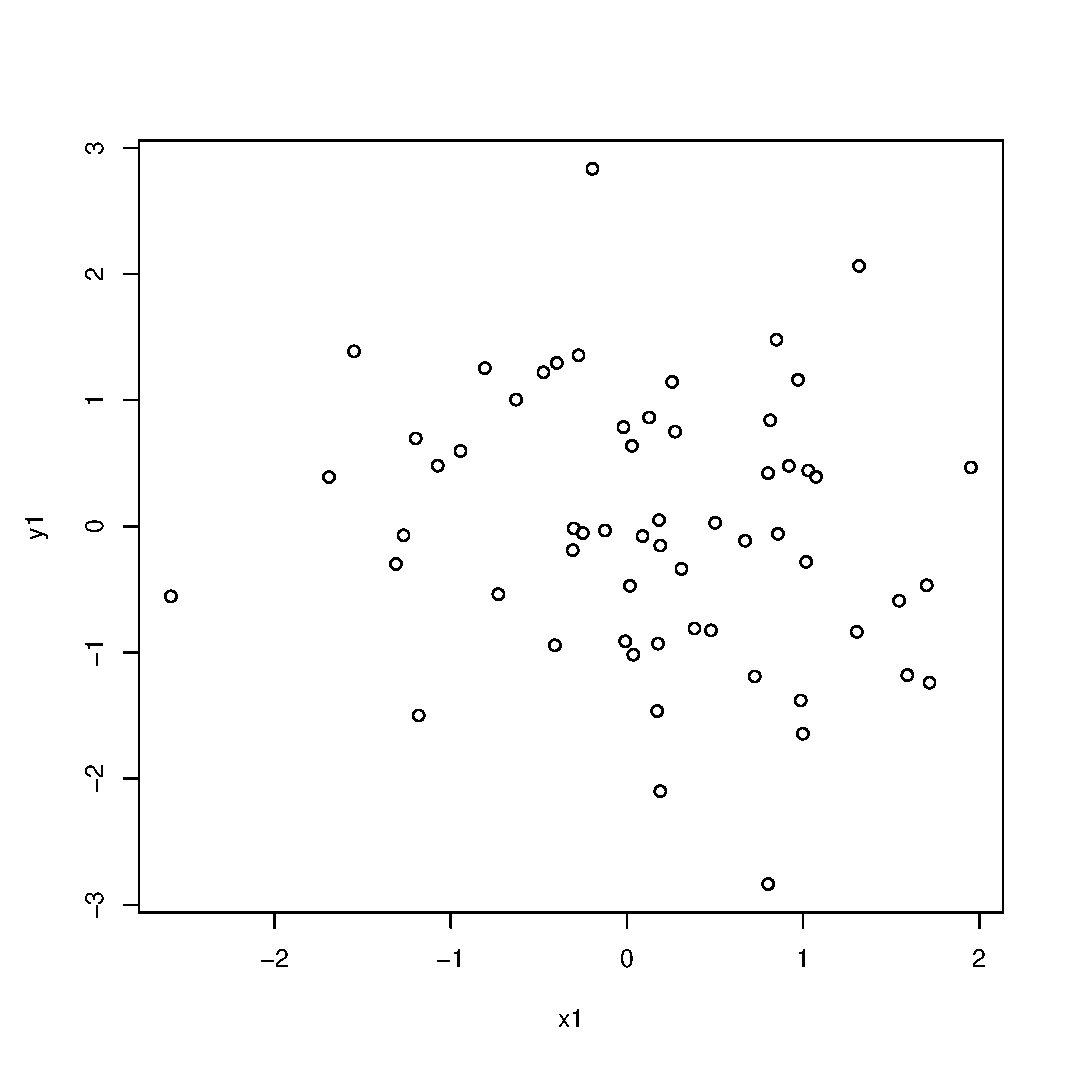
\includegraphics[width=8.2cm]{img/plot1.eps}
\end{center}
\end{breakbox}
このように先ほどと違い,点がバラバラである.
\begin{breakbox}
\begin{verbatim}
> result1=lm(y1~x1)
> result1

Call:
lm(formula = y1 ~ x1)

Coefficients:
(Intercept)           x1  
    0.01997     -0.18988  
\end{verbatim}
\end{breakbox}
この場合,回帰式は
\begin{eqnarray*}
Y&=&0.01997-0.18988X
\end{eqnarray*}
である.この回帰式を赤線でプロットしたものが下図である.
\begin{center}
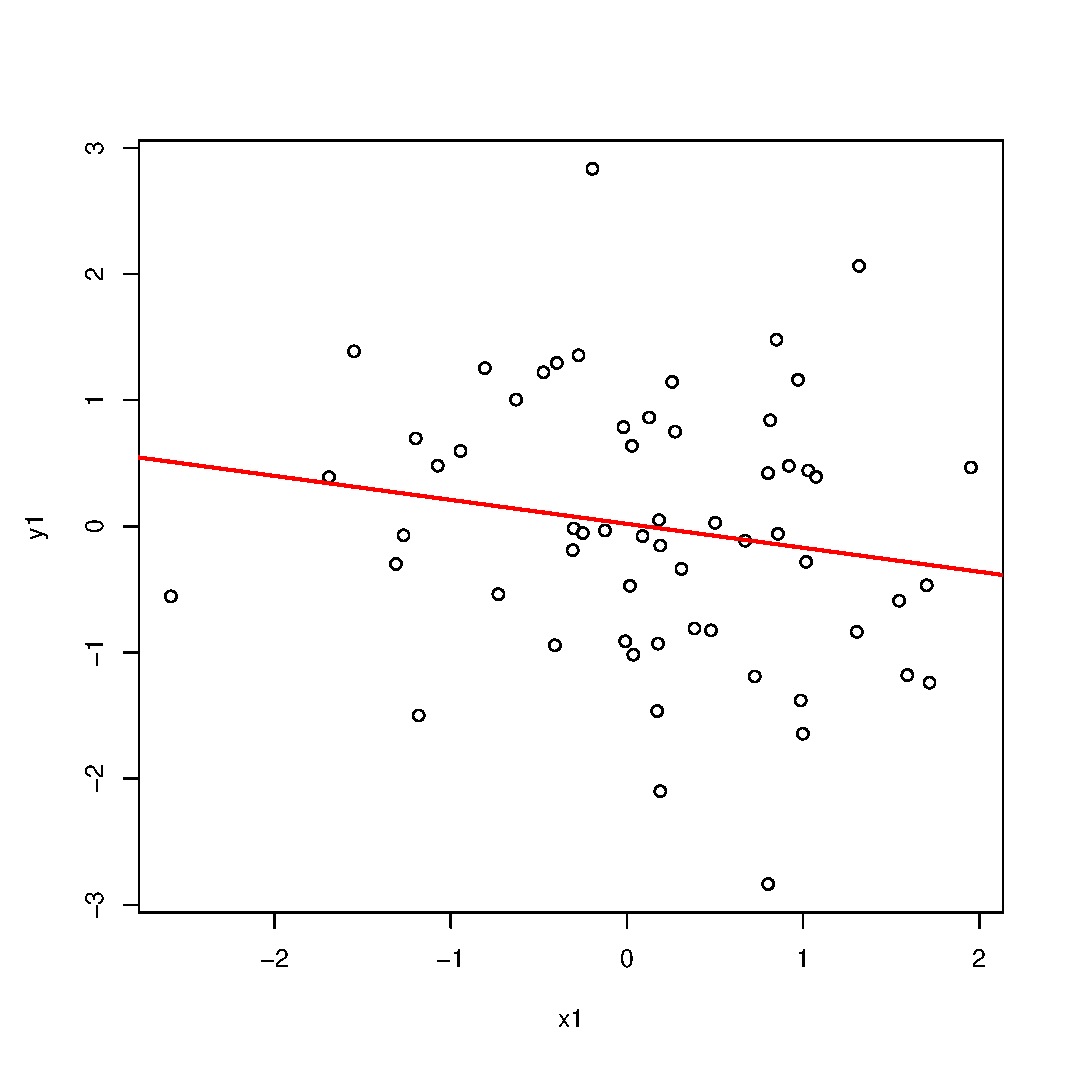
\includegraphics[width=8.2cm]{img/abline1.eps}
\end{center}

あまり意味のない線のように見える.そこで,先ほどと同様に分散分析表を確認する.
\begin{breakbox}
\begin{verbatim}
> summary(result1)

Call:
lm(formula = y1 ~ x1)

Residuals:
     Min       1Q   Median       3Q      Max 
-2.70223 -0.75451 -0.07851  0.76754  2.77611 

Coefficients:
            Estimate Std. Error t value Pr(>|t|)
(Intercept)  0.01997    0.13663   0.146    0.884
x1          -0.18988    0.14523  -1.307    0.196

Residual standard error: 1.044 on 58 degrees of freedom
Multiple R-squared: 0.02863,    Adjusted R-squared: 0.01188 
F-statistic: 1.709 on 1 and 58 DF,  p-value: 0.1962 
\end{verbatim}
\end{breakbox}
つまりこの結果は以下であり,
\begin{description}
\item[入力された式] \mbox{}\\
\verb+y1 ~ x1+
\item[残差の分布]\mbox{}\\
\begin{tabular}{ccccc}
\noalign{\hrule height 1pt}
最小値&25\%点&中央値&75\%点&最大値\\ \hline
-2.70223&-0.75451&-0.07851&0.76754& 2.77611 \\
\noalign{\hrule height 1pt}
\end{tabular}
\item[係数]\mbox{}\\
\begin{tabular}{rrrrr}
\noalign{\hrule height 1pt}
    &\multicolumn{1}{c}{推定値}&\multicolumn{1}{c}{標準誤差}&\multicolumn{1}{c}{t値}&\multicolumn{1}{c}{P-値($Pr( t_0>|t|)$)} \\ \hline
切片& 0.01997& 0.13663& 0.146&0.884 \\
  x1&-0.18988& 0.14523&-1.307&0.196 \\
\noalign{\hrule height 1pt}
\end{tabular}

帰無仮説が棄却されていないのがわかる.
\item[回帰統計]\mbox{}\\
\begin{tabular}{lr}
\noalign{\hrule height 1pt}
標準誤差&1.044(自由度58)\\
決定係数$R^2$&0.02863\\
自由度調整済決定係数$R^2$&0.01188\\
F値(観測された分散比)&1.709(自由度1と58)\\
P-値&0.1962\\
\noalign{\hrule height 1pt}
\end{tabular}

ここのP-値も大きい.
\end{description}
\subsubsection{{\tt lm}関数について}
{\tt lm}関数は以下のように使用する.
\begin{screen}
\begin{verbatim}
lm(formula , data,...)
\end{verbatim}
\end{screen}
\begin{description}
\item[{\tt formula}の指定方法] \mbox{} 
\begin{center}
\begin{tabular}{l|p{11.6cm}}
\noalign{\hrule height 1pt}
 \multicolumn{1}{c|}{{\tt formula}} & \multicolumn{1}{c}{回帰モデル式}\\ \hline
 \verb|y~x| &$y=\alpha +\beta x+\epsilon$ \\ 
 \verb|y~x1+x2| &$y=\alpha +\beta_1 x_1+\beta_2 x_2 +\epsilon$ \\ 
 \verb|y~x1*x2| & $y=\alpha +\beta_1 x_1+\beta_2 x_2+\beta_3 x_1 x_2+ +\epsilon$\\ 
 \verb|y~x1+x2+x1*x2| & \hspace{6em}〃\\ 
 \verb|y~(x1+x2)^2| & \hspace{6em}〃\\ 
 \verb|y~x-1| & $y=\beta x +\epsilon$ (定数項なし)\\ 
 \verb|y~x+0| & \hspace{6em}〃\\ 
 \verb|y~x+I(x^2)| & $y=\alpha+\beta_1 x+\beta_2 x^2+\epsilon$\\ 
 \verb|y~. , data=データ名| &指定したデータに含まれる{\tt y}を目的変数,{\tt y}以外の変数すべてを説明変数に指定する.($y=\alpha+\beta_1 x_1+\cdots+\beta_p x_p +\epsilon$) \\ 
\noalign{\hrule height 1pt}
\end{tabular}
\end{center}

なお,$\epsilon$は誤差項のことである.
\end{description}

lm関数が返すオブジェクトには,以下の情報が含まれるが特に覚える必要はない.
\begin{breakbox}
\begin{verbatim}
> result=lm(y2~x2)
> str(result)
List of 12
 $ coefficients : Named num [1:2] -0.0725 2.9873
  ..- attr(*, "names")= chr [1:2] "(Intercept)" "x2"
 $ residuals    : Named num [1:60] 0.6062 0.6405 -0.0037 0.7905 0.131 ...
  ..- attr(*, "names")= chr [1:60] "1" "2" "3" "4" ...
 $ effects      : Named num [1:60] 4.0488 24.4985 -0.0605 0.6912 0.0932 ...
  ..- attr(*, "names")= chr [1:60] "(Intercept)" "x2" "" "" ...
 $ rank         : int 2
 $ fitted.values: Named num [1:60] -4.272 -2.465 -0.381 -2.321 0.484 ...
  ..- attr(*, "names")= chr [1:60] "1" "2" "3" "4" ...
 $ assign       : int [1:2] 0 1
 $ qr           :List of 5
  ..$ qr   : num [1:60, 1:2] -7.746 0.129 0.129 0.129 0.129 ...
  .. ..- attr(*, "dimnames")=List of 2
  .. .. ..$ : chr [1:60] "1" "2" "3" "4" ...
  .. .. ..$ : chr [1:2] "(Intercept)" "x2"
  .. ..- attr(*, "assign")= int [1:2] 0 1
  ..$ qraux: num [1:2] 1.13 1.06
  ..$ pivot: int [1:2] 1 2
  ..$ tol  : num 1e-07
  ..$ rank : int 2
  ..- attr(*, "class")= chr "qr"
 $ df.residual  : int 58
 $ xlevels      : Named list()
 $ call         : language lm(formula = y2 ~ x2)
 $ terms        :Classes 'terms', 'formula' length 3 y2 ~ x2
  .. ..- attr(*, "variables")= language list(y2, x2)
  .. ..- attr(*, "factors")= int [1:2, 1] 0 1
  .. .. ..- attr(*, "dimnames")=List of 2
  .. .. .. ..$ : chr [1:2] "y2" "x2"
  .. .. .. ..$ : chr "x2"
  .. ..- attr(*, "term.labels")= chr "x2"
  .. ..- attr(*, "order")= int 1
  .. ..- attr(*, "intercept")= int 1
  .. ..- attr(*, "response")= int 1
  .. ..- attr(*, ".Environment")=<environment: R_GlobalEnv> 
  .. ..- attr(*, "predvars")= language list(y2, x2)
  .. ..- attr(*, "dataClasses")= Named chr [1:2] "numeric" "numeric"
  .. .. ..- attr(*, "names")= chr [1:2] "y2" "x2"
 $ model        :'data.frame':	60 obs. of  2 variables:
  ..$ y2: num [1:60] -3.666 -1.825 -0.385 -1.531 0.615 ...
  ..$ x2: num [1:60] -1.406 -0.801 -0.103 -0.753 0.186 ...
  ..- attr(*, "terms")=Classes 'terms', 'formula' length 3 y2 ~ x2
  .. .. ..- attr(*, "variables")= language list(y2, x2)
  .. .. ..- attr(*, "factors")= int [1:2, 1] 0 1
  .. .. .. ..- attr(*, "dimnames")=List of 2
  .. .. .. .. ..$ : chr [1:2] "y2" "x2"
  .. .. .. .. ..$ : chr "x2"
  .. .. ..- attr(*, "term.labels")= chr "x2"
  .. .. ..- attr(*, "order")= int 1
  .. .. ..- attr(*, "intercept")= int 1
  .. .. ..- attr(*, "response")= int 1
  .. .. ..- attr(*, ".Environment")=<environment: R_GlobalEnv> 
  .. .. ..- attr(*, "predvars")= language list(y2, x2)
  .. .. ..- attr(*, "dataClasses")= Named chr [1:2] "numeric" "numeric"
  .. .. .. ..- attr(*, "names")= chr [1:2] "y2" "x2"
 - attr(*, "class")= chr "lm"
\end{verbatim}
\end{breakbox}
\begin{description}
\item[返り値に含まれる主なオブジェクトとそれを利用する関数]\mbox{}\\
ここでは,\verb+result=lm(y2~x2)+とした場合の{\tt result}のことである.
\begin{itemize}
\item モデル式 \\
先ほど説明した {\tt formula}を指す.\verb+result$call+で取り出すことができる.
\item 係数 \\
\verb+result$coefまたは+\verb+result$coefficient+や\verb+coef(result)+で取り出すことができる.
\item 残差\\
観測値と推定したモデルとの誤差.\verb+result$residual+や\verb+result$residuals+や\verb+result$resid+や\\
\verb+residuals(result)+や\verb+resid(result)+で取り出すことができる.
\item 残差平方和\\
数式で表すと$\sum \limits ^n _{i=1} \left( y-\hat{y} \right)$.\verb+deviance(result)+で取り出すことができる.また,\verb+sum(result2$resid^2)+とするのと同じである.
\item 推定値\\
\verb+predict(result)+でモデルに当てはめた値,つまり$y_2$の推定値$\hat{y_2}$を得る.また,\verb+predict(result,newdata=データ名)+とすることで予測を行うこともできる.つまり,$\mbox{残差}=\mbox{観測値}-\mbox{推定値}$ということである.\\
※ データには回帰分析を行ったデータと同じ変数が存在する必要がある.
\item 作図\\
\verb+plot(result)+とすると4つ作図される.以下にそれぞれの説明を記す.
\end{itemize}
\begin{indentation}{3em}{0pt}
\begin{enumerate}
\item 残差と推定値の散布図\\
図の横軸が推測値,縦軸が残差である.この図から残差の全体像を確認することができる.
\begin{center}
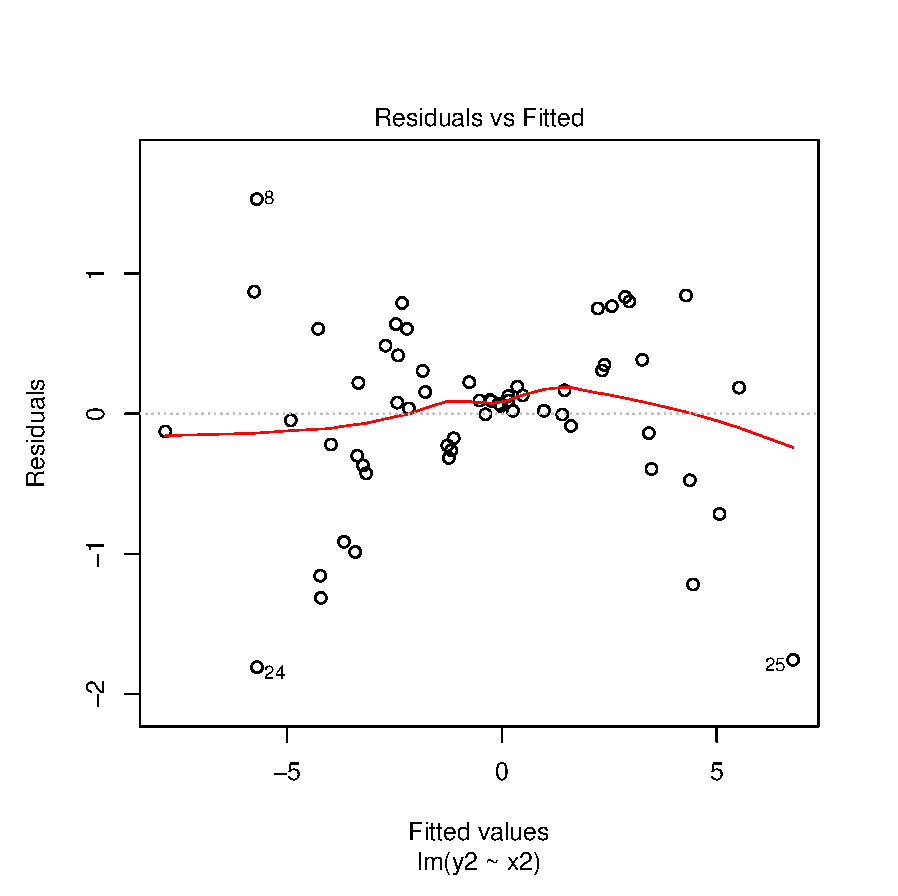
\includegraphics[width=11cm]{img/plotlm1.eps}
\end{center}
\item 残差の正規QQプロット\\
正規QQプロットじゃデータの正規性を考察するためにデータを視覚化する方法.データが正規分布に従う場合,点が一直線上に並べられる.
\begin{center}
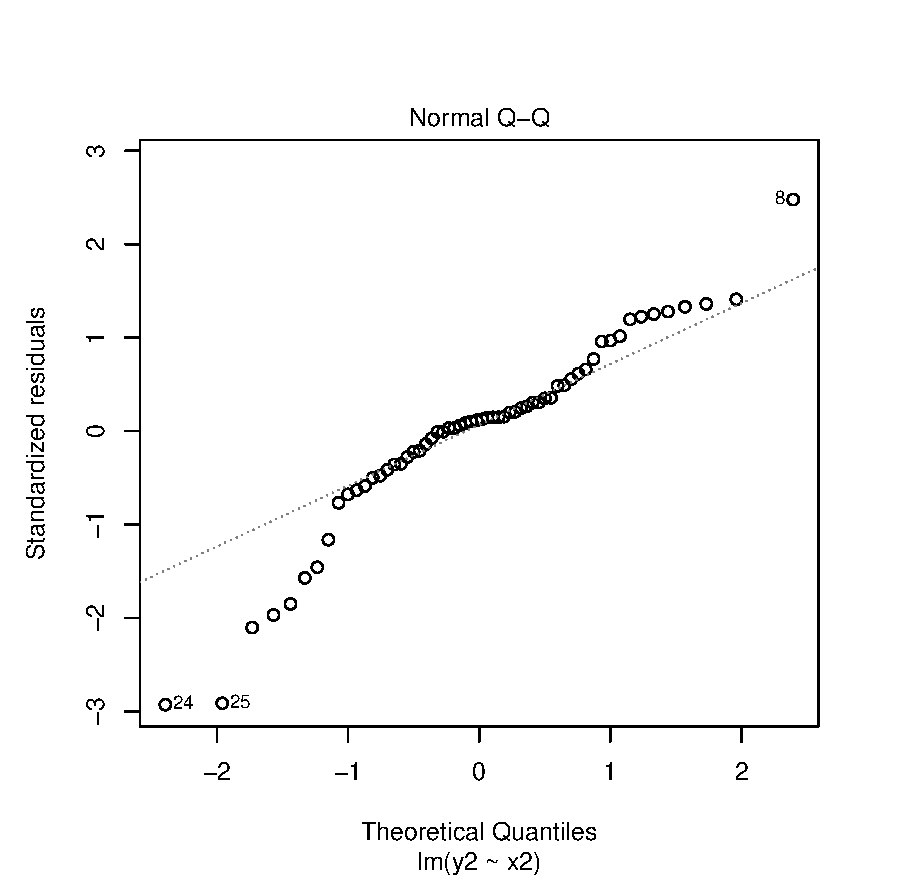
\includegraphics[width=11cm]{img/plotlm2.eps}
\end{center}
\item Scale-Location図\\
標準化した残差の絶対値の平方根を縦軸にし,推測値を横軸とした散布図.
\begin{center}
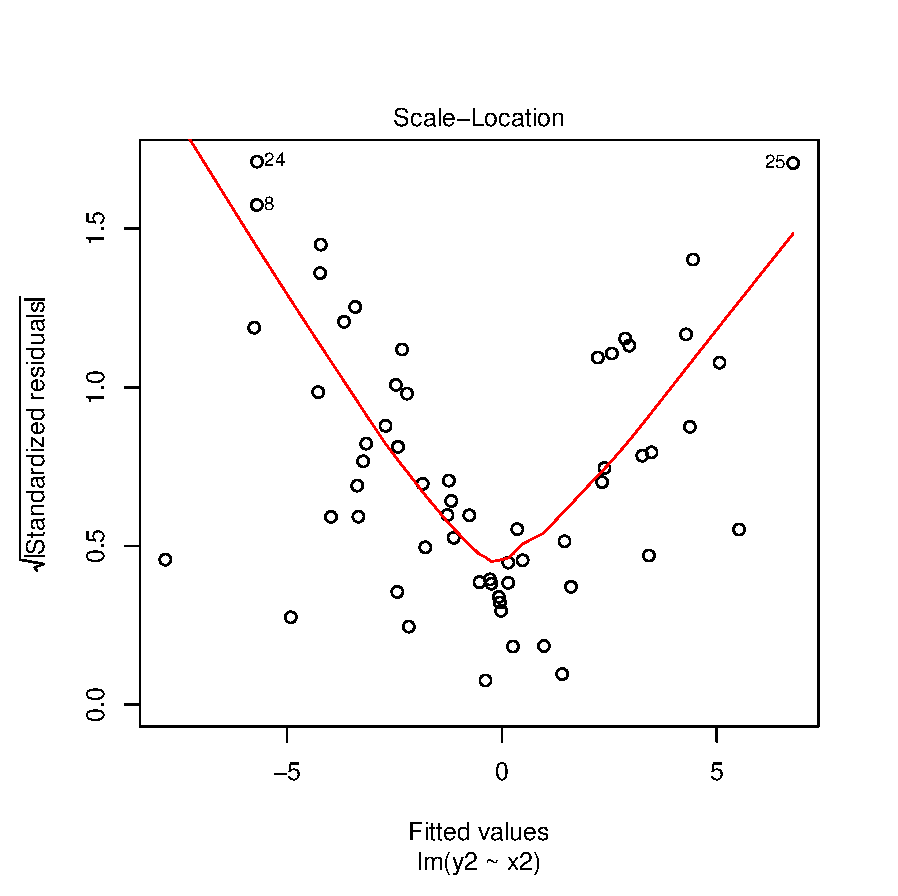
\includegraphics[width=11cm]{img/plotlm3.eps}
\end{center}
\item 残差-てこ比\\
てこ比は観測値が推測値に及ぼす影響の大きさである.クックの距離は,各データがどれだけ推定に影響を与えているかを示す指標.
\begin{center}
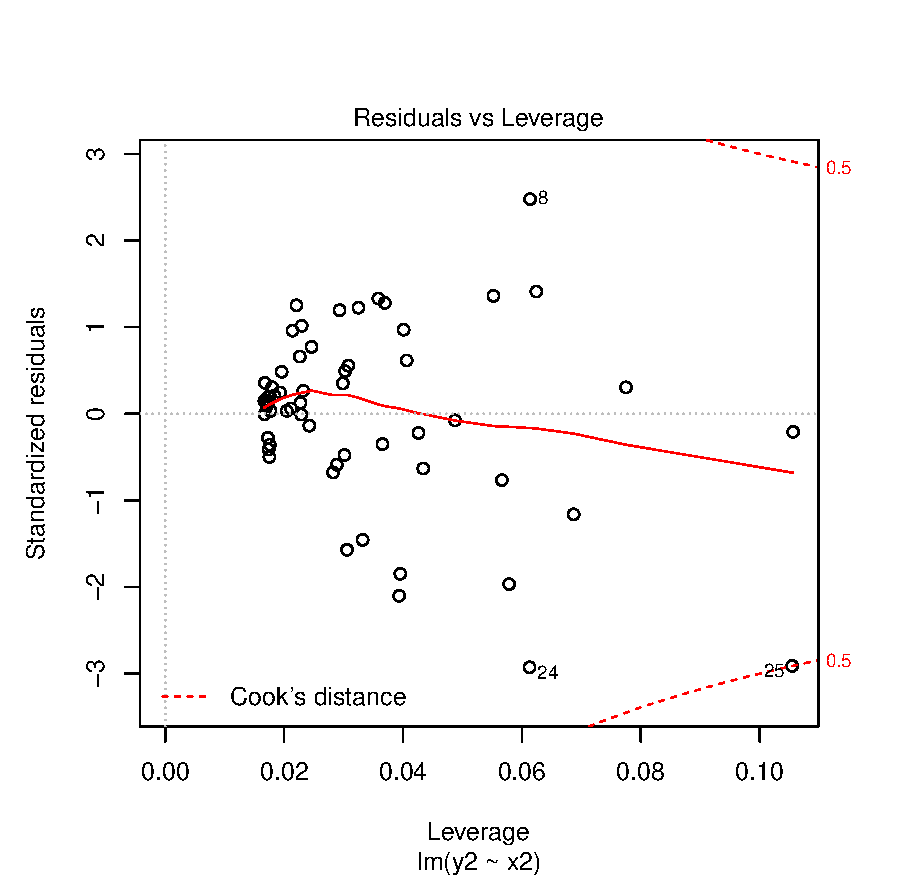
\includegraphics[width=11cm]{img/plotlm4.eps}
\end{center}
\end{enumerate}
\end{indentation}
\end{description}
\subsubsection{補遺}
\begin{description}
\item[平均]\mbox{}\\
\begin{eqnarray*}
\bar{x}&=&\frac{1}{n}\sum \limits ^n_{i=1}x_i
\end{eqnarray*}
\item[分散]\mbox{}\\
\begin{eqnarray*}
s^2 &=& \frac{1}{n} \sum_{i=1}^{n}(x_i - \bar{x})^2 \\
    &=& \bar{x^2}-\left( \bar{x} \right)^2
\end{eqnarray*}
これを{\bf 標本分散}という.
\item[不偏分散]\mbox{}\\
上記の分散は,$\displaystyle E[s^2] = \frac{n-1}{n} \sigma^2 (\sigma^2\mbox{は母集団の分散})$とした場合,標本の分散は母集団の分散よりも小さくなる傾向がある.すなわち,標本の分散は母集団の分散の不偏推定量ではない.不偏分散は以下の式で表される.また,Rの{\tt var}関数では不偏分散が採用されている.標本数が十分に大きければ標本分散とほぼ等しくなる.
\begin{eqnarray*}
u^2 &=& \frac{1}{n-1} \sum_{i=1}^{n}(x_i - \bar{x})^2 
\end{eqnarray*}
\item[標準偏差]\mbox{}\\
\begin{eqnarray*}
\sqrt{\mathrm{V}(X)}
\end{eqnarray*}
つまり,分散の正の平方根.
\item[共分散]\mbox{}\\
\begin{eqnarray*}
\mathrm{Cov}(X, Y)&=&\frac{1}{n}\sum_{i=1}^{n} (x_{i}-\bar{x})(y_{i}-\bar{y})\\
&=& \frac{S_{xy}}{n}
\end{eqnarray*}
\item[相関係数]\mbox{}\\
\begin{eqnarray*}
\mathrm{Cor}(X,Y)&=&\frac{\mathrm{Cov}(X,Y)}{\sqrt{\mathrm{V}(X)}\sqrt{\mathrm{V}(Y)}}\\
&=&\frac{ \displaystyle \sum_{i=1}^{n} (x_{i}-\bar{x})(y_{i}-\bar{y}) }{ \displaystyle \sqrt{\sum_{i=1}^n(x_{i}-\bar{x})^2} \sqrt{\sum_{i=1}^n(y_{i}-\bar{y})^2}}
\end{eqnarray*}
つまり,共分散をそれぞれの標準偏差で割ったもの.
\item[最小二乗法]\mbox{}\\
$y_i$の推定値を$\hat{y_i}=\alpha+\beta x_i$とした場合,実際の観測値と推定値の差を残差と呼ぶ.残差を$e_i$
で表すと,
\begin{eqnarray*}
e_i&=&y_i-\hat{y}\\
&=&y_i-\left( \alpha+\beta x_i \right)
\end{eqnarray*}
であり,最小二乗法は残差平方和を最小にする方法である.残差平方和を$\alpha$と$\beta$の関数とみなすと以下のように表せる.
\begin{eqnarray*}
S_e(\alpha,\beta)&=&\sum \limits ^n _{i=1}e_i ^2\\
&=&\sum \limits ^n _{i=1}\left( y_i-\alpha-\beta x_i \right)
\end{eqnarray*}
$S(\alpha,\beta)$は$\alpha,\beta$に関する2次関数で,$S(\alpha,\beta)$を最小化する$\alpha,\beta$を見つけるには微分すれば良い.

まず,$\alpha$に関して微分する.
\begin{eqnarray*}
\frac{\partial S}{\partial \alpha}&=&-2\sum\limits ^n_{i=1}\left( y_i-\alpha-\beta x_i \right)=0
\end{eqnarray*}
これを変形する.
\begin{eqnarray*}
\sum\limits ^n_{i=1}y_i&=&\sum\limits ^n_{i=1}\alpha+\sum\limits ^n_{i=1}\beta x_i
\end{eqnarray*}
両辺を$n$で割る.
\begin{eqnarray}
\bar{y}&=&\alpha+\beta\bar{x} \label{alpha}
\end{eqnarray}
また,$\beta$に関して微分する.
\begin{eqnarray*}
\frac{\partial S}{\partial \beta}&=&-2\sum\limits ^n_{i=1}\left( y_i-\alpha-\beta x_i \right)x_i=0
\end{eqnarray*}
変形し,
\begin{eqnarray}
\sum\limits ^n_{i=1}x_i y_i&=&\alpha \sum\limits ^n_{i=1}x_i+\beta\sum\limits ^n_{i=1}\beta x_i^2 \label{beta}
\end{eqnarray}
(\ref{alpha})(\ref{beta})の連立方程式より$\alpha$と$\beta$について解く.(\ref{alpha})を$\alpha$について解き,(\ref{beta})に代入する.
\begin{eqnarray*}
\sum \limits ^n_{i=1}x_i y_i&=&\left( \bar{y}-\beta \bar{x} \right)\sum \limits ^n_{i=1}x_i +b\sum \limits ^n_{i=1}x_i^2 \\
&=&n\bar{x}\bar{y}+b\left( \sum \limits ^n_{i=1}x_i^2 - n\bar{x}^2 \right)
\end{eqnarray*}
また,以下の式が得られる.
\begin{eqnarray*}
S_{xy}&=&\beta S_{xx}
\end{eqnarray*}
ただし,$S_{xx}$と$S_{xy}$は以下である.
\begin{eqnarray*}
S_{xx}&=&\sum \limits^n _{i=1}\left( x_i -\bar{x} \right)^2=\sum \limits^n _{i=1}x_i^2-n\bar{x}\\
S_{xy}&=&\sum \limits^n _{i=1}\left( x_i-\bar{x} \right)\left( y_i - \bar{y} \right)=\sum \limits^n _{i=1}x_i y_i -n\bar{x}\bar{y}
\end{eqnarray*}
以上より,(\ref{estalpha})と(\ref{estbeta})を得る.
\begin{eqnarray}
\alpha&=&\bar{y}-b\bar{x} \label{estalpha}\\
\beta  &=&\frac{S_{xy}}{S_{xx}} \label{estbeta}
\end{eqnarray}
また,細かな計算は省略するが行列計算を行うことで,最小二乗法によって係数を求めることもできる.
$Y$を目的変数の$n$行1列の行列としてとして,$X$を説明変数の$n$行2列\footnote[1]{この行列$X$の左に成分がすべて1の行を結合して定数項を推定している.}として,$Y=X\beta$となる行列$\beta$を求める.
\begin{eqnarray*}
\beta=(X^T X)^{-1}X^T Y
\end{eqnarray*}
Rでは\verb+beta=solve(t(x)%*%x)%*%t(x)%*%y+と表現する.
\item[決定係数]\mbox{}\\
残差平方和を$S_e=\sum \limits^n _{i=1} e_i^2$とする.目的変数$y$の偏差平方和を$S_{yy}=\sum \limits^n _{i=1}\left( y_i -\bar{y} \right)^2=\sum \limits^n _{i=1}y_i^2-n\bar{y}$とする.
\begin{eqnarray*}
R^2&=&1-\frac{S_E}{S_{yy}}
\end{eqnarray*}
また,寄与率とも言う.説明変数が目的変数をどの程度説明できるかを表す.標本値から求めた回帰方程式のあてはまりの良さの尺度である.
\item[自由度調整済み決定係数]\mbox{}\\
説明変数を増やすと決定係数は大きくなるため,サンプル数を$n$,データの中の説明変数の数を$k$として,自由度を調整した決定係数が以下である.
\begin{eqnarray*}
(adjusted\ R^2)&=&1-\frac{S_E /(n-k-1)}{S_{yy} /(n-1)}
\end{eqnarray*}
\item[標準誤差]\mbox{}\\
残差の不偏分散を以下とする.
\begin{eqnarray*}
S_e^2&=&\frac{S_e}{n-k-1}
\end{eqnarray*}
係数$\alpha$,$\beta$の標準誤差SE$(\alpha)$,$SE(\beta)$は以下で求められる.
\begin{eqnarray*}
SE(\alpha)&=&\sqrt{S_e^2 \left[\frac{1}{n}+\frac{\bar{x}^2}{\sum \limits ^n _{i=1}\left( x_i-\bar{x} \right)}\right]}\\
SE(\beta)&=&\sqrt{\frac{S_e^2}{\sum \limits ^n _{i=1}\left( x_i-\bar{x} \right)}}
\end{eqnarray*}
\item[t値]\mbox{}\\
係数$\alpha$,$\beta$のt値は以下である.
\begin{eqnarray*}
t_\alpha &=&\frac{\alpha}{SE(\alpha)}\\
t_\beta &=&\frac{\beta}{SE(\beta)}
\end{eqnarray*}
このt値に対応するp値は{\tt pt}関数で求めることができる.t値は帰無仮説:係数が0であるという仮説検定の統計量である.p値が有意水準(0.05,0.01,0.005)よりも小さい場合は,p値の右側にそれぞれ(*,**,***)を付ける.
\item[F値]\mbox{}\\
F値は帰無仮説:すべての係数が0であるという仮説検定の統計量である.F値は決定係数から求められ,自由度$k$,$n-k-1$のF分布に従う.
\begin{eqnarray*}
F&=&\frac{R^2}{1-R^2}\times\frac{n-k-1}{k}
\end{eqnarray*}
\end{description}\end{document}